\secslide{Documentation}

\begin{frame}{Why Should We Document Our Code?}
  \begin{center}
    \huge\textcolor{ccyan!90!cblack}{Well documented code improves\dots}
  \end{center}
  \begin{itemize}
    \item Maintainability: Future developers, debugging, \dots
    \item Accessibility: Make your package easier to understand for new users
    \item Collaboration: Docs as a shared knowledge source
  \end{itemize}
\end{frame}

\begin{frame}[fragile]{Tool Of Choice: Sphinx}
  \begin{columns}[t, onlytextwidth]
    \begin{column}{0.68\textwidth}
      \begin{itemize}
        \setlength{\itemsep}{1em}
        \item FOSS, extensible documentation generator written in Python
        \item Multiple output formats: \texttt{HTML}, \LaTeX, ePub, and more\dots
        \item Content is written using a mark-up language (\texttt{reST} or \texttt{MyST})
        \item Support for various docstring formats (some through extensions)
        \item Install via uv or mamba:
          \begin{minted}{text}
            $ uv pip install sphinx
            $ mamba install sphinx
          \end{minted}
      \end{itemize}
    \end{column}
    \hfill
    \begin{column}{0.38\textwidth}
      \begin{center}
      
\includegraphics[width=0.8\textwidth]{logos/sphinx-logo.pdf}
      \end{center}
    \end{column}
  \end{columns}
\end{frame}


{
\usemintedstyle{code-light}
\begin{frame}[fragile]{Getting Started}
  \begin{minted}[escapeinside=||]{shell-session}
    $ sphinx-quickstart docs
    |\textcolor{ccyan}{> Separate source and build directories (y/n) [n]:}| y
    |\textcolor{ccyan}{> Project name:}| ...
    |\textcolor{ccyan}{> Author name(s):}| ...
    |\textcolor{ccyan}{> Project release []:}| ...
    |\textcolor{ccyan}{> Project language [en]:}| ...
  \end{minted}

  \begin{center}
  \pause
  \begin{minipage}{.45\textwidth}
  \adjustbox{max height=5.5cm}{%
    \begin{forest}
      for tree={dir tree}
      [docs, opened
        [build, closed]
        [source, opened
          [\_static, closed]
          [\_templates, closed]
          [conf.py, pythonfile]
          [index.rst, textfile]
        ]
        [make.bat, batchfile]
        [Makefile, makefile]
      ]
    \end{forest}
  }
  \end{minipage}
  \hfill
  \pause
  \begin{minipage}{.45\textwidth}
    \adjustbox{max height=5.5cm}{%
      \begin{forest}
        for tree={dir tree}
        [docs, opened
          [\_build, closed]
          [\_static, closed]
          [\_templates, closed]
          [conf.py, pythonfile]
          [index.rst, textfile]
          [make.bat, batchfile]
          [Makefile, makefile]
        ]
      \end{forest}
    }
  \end{minipage}
  \end{center}
\end{frame}
}

{
\setbeamercolor{description item}{fg=cblack}
\begin{frame}[fragile]{Breakdown of the Generated Structure}
  \begin{description}[labelwidth=\widthof{\faFolderOpen \texttt{\_templates}}]
    \setlength{\itemindent}{-4em}
    \item [\textcolor{dircolor}{\faFolderOpen} \texttt{build}:] Output directory for the docs.
    \item [\textcolor{dircolor}{\faFolderOpen} \texttt{\_static}:] Directory for static elements such as images, icons, or logos.
    \item [\textcolor{dircolor}{\faFolderOpen} \texttt{\_templates}:] Used to store \iref{https://jinja.palletsprojects.com/en/stable/}{\texttt{Jinja}}
      templates for HTML page generation. %Also used by some Sphinx extensions.
    \item [\faFile* \texttt{index.rst}:] Root document; contains the root of the table of contents tree.
      % Effectively your landing page in the HTML version.
    \item [\faPython \texttt{conf.py}:] Main configuration file written in Python.
  \end{description}
\end{frame}
}

{
\usemintedstyle{code-light}
\begin{frame}[fragile]{Let's Build Our Docs}
  We will use the \texttt{Makefile} generated by \mintinline{shell-session}+sphinx-quickstart+ to build any format:
  \begin{minted}{shell-session}
    $ make <format>
  \end{minted}
  So, for the HTML version:
  \begin{minted}{shell-session}
    $ make html
  \end{minted}
  This will generate the HTML files for our docs inside the \texttt{build} directory.
  We can view the docs locally by running a Python HTTP server (in this case from inside the \texttt{docs} directory):
  \begin{minted}{shell-session}
    $ python -m http.server -d build/html [port]
  \end{minted}

  \begin{block}{Note}
    \mintinline{shell-session}+[port]+ is optional, see \mintinline{shell-session}+python -m http.server --help+.
  \end{block}
\end{frame}
}

\begin{darkframe}[fragile]{Setting Up conf.py}
  The \texttt{conf.py} file generated by Sphinx should look something like this:
  \begin{minted}{python}
    # -- Project information ------------------------
    project = 'pyopp'
    copyright = '2025, Author'
    author = 'Author'
    release = 'v0.1'

    # -- General configuration ----------------------
    extensions = []

    templates_path = ['_templates']
    exclude_patterns = []

    # -- Options for HTML output --------------------
    html_theme = 'alabaster'
    html_static_path = ['_static']
  \end{minted}
\end{darkframe}


\begin{darkframe}[fragile]{Setting Up conf.py | Project Information}
  \vspace*{0.25cm}
  Let's get some metadata from \texttt{pyproject.toml} using \texttt{tomli} or \texttt{tomllib} (Python $\geqslant$ \texttt{3.11}):\\[0.25\baselineskip]
  \footnotesize
  \begin{minted}{python}
    #!/usr/bin/env python3
    import datetime
    import sys
    from pathlib import Path

    import package                                                           # your package

    if sys.version_info < (3, 11):
        import tomli as tomllib
    else:
        import tomllib

    pyproject_path = Path(__file__).parent.parent.parent / "pyproject.toml"  # Get path of pyproject.toml
    pyproject = tomllib.loads(pyproject_path.read_text())                    # Load contents

    project = pyproject["project"]["name"]                                   # Get project name
    author = pyproject["project"]["authors"][0]["name"]                      # Get author name
    copyright = "{}.  Last updated {}".format(
        author, datetime.datetime.now().strftime("%d %b %Y %H:%M")
    )                                                                        # Set copyright string
    python_requires = pyproject["project"]["requires-python"]                # Get minimum python version requirement
    rst_epilog = f"""
    .. |python_requires| replace:: {python_requires}
    """                                                                      # Make python_requires var accessible

    version = package.__version__                                            # Get version
    release = version                                                        # Full release version
  \end{minted}
\end{darkframe}


\begin{darkframe}[fragile]{Setting Up conf.py | General Configuration}
  Sphinx extensions add functionality and customization. The following extensions
  are some of the extensions we always use in our docs:\\[0.25\baselineskip]
    \small
    \begin{minted}{python}
      extensions = [
          "sphinx.ext.autodoc",                # Imports modules and pulls in documentation from docstrings
          "sphinx.ext.intersphinx",            # Cross-references to other projects
          "sphinx.ext.coverage",               # Collects doc coverage stats
          "sphinx.ext.viewcode",               # Links to highlighted source code (i.e. "[source]" button)
          "sphinx_automodapi.automodapi",                    # Automatically generates module documentation
          "sphinx_automodapi.smart_resolver",                # Helps resolving some imports
          "numpydoc",                                        # Support for the NumPy docstring format
          "IPython.sphinxext.ipython_console_highlighting",  # Syntax highlighting of ipython prompts
          "sphinx_copybutton",                               # Adds a copybutton to code blocks
      ]
    \end{minted}
\end{darkframe}

{
\usemintedstyle{code-light}
\begin{frame}[fragile]{Setting Up \texttt{conf.py} | General Configuration}
    Some extensions are not shipped with Sphinx and need to be installed separately in your environment:
    \begin{minted}{shell-session}
      $ mamba install sphinx-automodapi numpydoc pydata-sphinx-theme sphinx-copybutton
    \end{minted}
    or with \texttt{uv}
    \begin{minted}{shell-session}
      $ uv pip install sphinx-automodapi numpydoc pydata-sphinx-theme sphinx-copybutton
    \end{minted}
\end{frame}
}

\begin{darkframe}[fragile]{Setting Up conf.py | General Configuration}
  Now we can set up some more settings for the extensions:\\[0.25\baselineskip]
    \begin{minted}{python}
    # gets rid of some errors during build
    numpydoc_show_class_members = False
    numpydoc_class_members_toctree = False

    intersphinx_mapping = {
       "numpy": ("https://numpy.org/doc/stable", None),
       ...
    }

    suppress_warnings = ["intersphinx.external"]  # sometimes necessary

    templates_path = ["_templates"]
    exclude_patterns = ["build", "Thumbs.db", ".DS_Store", "changes", "*.log"]

    source_suffix = {".rst": "restructuredtext"}  # Set .rst files as source files for docs
    master_doc = "index"                          # index.rst as root file
  \end{minted}
\end{darkframe}

\begin{darkframe}[fragile]{Setting Up conf.py | HTML And Theme Options}
  HTML options set the look of your docs. The Sphinx community has created a variety of
  themes you can choose from.\\[0.25\baselineskip]
  \begin{minted}{python}
    html_theme = "pydata_sphinx_theme"            # Modern, widely used theme

    html_static_path = ["_static"]
    html_favicon = "_static/favicon/favicon.ico"  # Icon file for browser tabs
    html_css_files = ["custom.css"]               # Custom CSS settings like colors or fonts
    html_file_suffix = ".html"

    html_theme_options = {...}                    # Depends on the theme

    html_title = f"{project}"                     # e.g. your project name
    htmlhelp_basename = project + " docs"
  \end{minted}
  \vspace{0.25\baselineskip}
  Check out \emph{Sphinx Themes Gallery} for a curated list of available themes:
  \iref{https://sphinx-themes.org/}{sphinx-themes.org}
\end{darkframe}


\begin{darkframe}[fragile]{Filling the Docs: Landing Page}
    \footnotesize
    \begin{minted}{rst}
      :html_theme.sidebar_secondary.remove: true
      :html_theme.sidebar_primary.remove: true

      .. _package:

      =======
      Package
      =======

      .. currentmodule:: package

      **Version**: |version| | **Date**: |today|

      **Useful links**: `Source Repository <https://github.com/your_project/package>`__ |
      `Issue Tracker <https://github.com/your_project/package/issues>`__ |
      `Pull Requests <https://github.com/your_project/package/pulls>`__

      **License**: `MIT <https://github.com/your_project/package/blob/main/LICENSE>`__

      **Python**: |python_requires|

      .. toctree::
         :maxdepth: 1
         :hidden:

         api-reference/index
         changelog
    \end{minted}
\end{darkframe}


\begin{frame}[fragile]{Filling the Docs: API References}
  We will create the API references (semi-)automatically in a few steps:
  \begin{columns}[onlytextwidth]
    \begin{column}{0.48\textwidth}
      \begin{enumerate}
        \item <1-> Copy the structure of your actual package
        \item <2-> Populate every subdirectory with a \texttt{index.rst}
        \item <3-> Create separate \texttt{.rst} files for every submodule
      \end{enumerate}
      \vspace{0.25cm}
      \begin{center}
        \adjustbox{max height=5cm}{%
          \begin{forest}
            for tree={dir tree}
            [package, opened
              [module1, opened
                [\_\_init\_\_.py, pythonfile]
                [submodule\_a.py, pythonfile]
                [submodule\_b.py, pythonfile]
              ]
              [module2, opened
                [\_\_init\_\_.py, pythonfile]
                [submodule\_c.py, pythonfile]
              ]
              [\_\_init\_\_.py, pythonfile]
            ]
          \end{forest}
        }
      \end{center}
    \end{column}
    \begin{column}{0.48\textwidth}
      \begin{center}
        % \adjustbox{max height=5cm}{%
          \begin{forest}
            for tree={dir tree}
            [docs, opened
              [api-reference, opened
                [module1, opened
                  [index.rst, textfile, visible on=<2->]
                  [submodule\_a.rst, textfile, visible on=<3->]
                  [submodule\_b.rst, textfile, visible on=<3->]
                ]
                [module2, opened
                  [index.rst, textfile, visible on=<2->]
                  [submodule\_c.rst, textfile, visible on=<3->]
                ]
                [index.rst, textfile, visible on=<2->]
              ]
              [...]
            ]
          \end{forest}
        % }
      \end{center}
    \end{column}
  \end{columns}
\end{frame}


\begin{darkframe}[fragile]{Filling the Docs: API References}
  For now, the API reference will still be empty. We have to fill in
  the \texttt{index.rst} files to change that. Starting with
  \texttt{api-reference/index.rst}:\\[1em]

  \begin{columns}[onlytextwidth]
    \begin{column}{0.38\textwidth}
      \begin{minted}{rst}
        .. _api-reference:

        *************
        API Reference
        *************

        .. toctree::
          :maxdepth: 1
          :glob:

          */index
      \end{minted}
    \end{column}
    \hfill
    \begin{column}{0.58\textwidth}
      We add\dots
      \begin{enumerate}
        \setlength{\itemsep}{1.5em}
        \item A tag \texttt{.. \_api-reference:} to the file so we can reference it if necessary
        \item A title, \eg, \enquote{API Reference}
        \item The table of contents with the \texttt{.. toctree::} directive
          \begin{itemize}
            \item And add only \texttt{index.rst} files from the subdirectories to the TOC
          \end{itemize}
      \end{enumerate}
    \end{column}
  \end{columns}
\end{darkframe}

\begin{darkframe}[fragile]{Filling the Docs: API References}

  \begin{columns}[onlytextwidth]
    \begin{column}{0.52\textwidth}
      \scriptsize
      \begin{minted}{rst}
        .. _module1:

        ********************************
        Module1 (:mod:`package.module1`)
        ********************************

        .. currentmodule:: package.module1

        Introduction
        ============

        :mod:`package.module1` contains useful methods and classes.

        Submodules
        ==========

        .. toctree::
          :maxdepth: 1
          :glob:

          submodule_a
          submodule_b

        Reference/API
        =============

        .. automodapi:: package.module1
            :no-inheritance-diagram:
      \end{minted}
    \end{column}
    \hfill
    \begin{column}{0.46\textwidth}
      Now, we do the same for the \texttt{index.rst} files in the module directories:\\[1em]
      We add\dots
      \begin{enumerate}
        \setlength{\itemsep}{1.5em}
        \item A tag and module title
        \item The \texttt{.. currentmodule::} directive to let Sphinx know that
          classes and functions documented from here on are in the given module
        \item (optional) Some introduction to the module
        \item The table of contents for the submodules of the module
        \item The \texttt{.. automodapi::} directive for the current module to get a list of
          classes and functions
      \end{enumerate}
    \end{column}
  \end{columns}
\end{darkframe}

\begin{darkframe}[fragile]{Filling the Docs: API References}
  Finally, we write the submodule \texttt{.rst} files:

  \begin{columns}[onlytextwidth]
    \begin{column}{0.5\textwidth}
      \footnotesize
      \begin{minted}{rst}
        .. _submodule_a:

        ************************************************
        submodule_a (:mod:`package.module1.submodule_a`)
        ************************************************

        .. currentmodule:: package.module1.submodule_a

        Submodule of :mod:`package.module1`.


        Reference/API
        =============

        .. automodapi:: package.module1.submodule_a
            :inherited-members:
      \end{minted}
    \end{column}
    \hfill
    \begin{column}{0.46\textwidth}
      We add\dots
      \begin{enumerate}
        \setlength{\itemsep}{1.5em}
        \item A tag, the submodule title, and the\\\texttt{.. currentmodule::} directive
        \item (optional) Some introduction to the submodule
        \item The \texttt{.. automodapi::} directive for the current submodule to get a list of
          classes and functions
      \end{enumerate}
    \end{column}
  \end{columns}
\end{darkframe}

{
\usemintedstyle{code-light}
\begin{frame}[fragile]{reST: Headings}
  \begin{columns}[t, onlytextwidth]
    \begin{column}{0.33\textwidth}
        \begin{minted}{rst}
          ####
          Part
          ####

          *******
          Chapter
          *******

          Section
          =======

          Subsection
          ----------

          Subsubsection
          ^^^^^^^^^^^^^

          Paragraph
          """""""""
        \end{minted}
    \end{column}
    \hfill
    \begin{column}{0.66\textwidth}
      \begin{itemize}
        \setlength{\itemsep}{1.5em}
        \item The structure is technically determined by order of occurance
        \begin{itemize}
          \item \textbf{But}: For better readability stick to the same order throughout your docs, \eg, the one shown here (recommended)
        \end{itemize}
        \item While overlines are optional, they are encouraged for parts and chapters
        \item Any of the following symbols are valid for over- and underlines:\\
          \textcolor{cpink}{\texttt{\#} \texttt{*} \texttt{=} \texttt{-} \texttt{\textasciicircum} \texttt{"} \texttt{+} \texttt{\_} \texttt{\textasciitilde}}
          \mintinline{text}{` . , : ; ' ! ? & $ %}
          \mintinline{text}+( ) [ ] { }+\\
          \mintinline{text}+< > @ \ / |+
      \end{itemize}
    \end{column}
  \end{columns}
\end{frame}

\begin{frame}[fragile]{reST: Roles, Directives, and Field Lists}
  \begin{itemize}
    \setlength{\itemsep}{1em}
    \item Roles are \textbf{inline} pieces of explicit markup that are understood by Sphinx.
    The syntax is:
    \begin{center}
      \begin{minted}{rst}
        :rolename:`content`
      \end{minted}
    \end{center}

  \item [\to] Examples:
    \begin{minted}{rst}
      :mod:`package.module1` :code:`foo = 42` :math:`F = m\cdot a`
    \end{minted}

  \item Directives are \textbf{blocks} of explicit markup that are understood by Sphinx.
    The syntax is:
    \begin{center}
      \footnotesize
      \begin{minted}{rst}
        .. directive:: [(optional) arguments]
           [:(optional) field list:] [(optional) field list value]

           [Body elements of the directive]
      \end{minted}
    \end{center}

  \item [\to] Examples:
    \footnotesize
    \begin{minted}{rst}
      .. image:: picture.png
         :width: 90%
         :alt: A nice picture.

      .. code-block::
         :caption: A code block.

         def func(param: int) -> int: ...
    \end{minted}
  \end{itemize}
\end{frame}
}

\begin{frame}[fragile]{Hosting on \rtd}
  \begin{itemize}
    \setlength{\itemsep}{1.5em}
    \item Free, if your package is open-source, \ie, publically available on, \eg, GitHub or GitLab and
      no handling of secrets required
    \item Allows you to preview your docs on every PR
    \item Works seamlessly with Sphinx
    \item Automatically builds the docs from your \texttt{main} branch
    \item Supports downloading the docs in PDF or other formats
  \end{itemize}
\end{frame}

\begin{darkframe}[fragile]{Hosting on \rtd}
  \begin{enumerate}
    \item Set up a \texttt{.readthedocs.yaml} file in your repository:
        \begin{minted}{yaml}
          version: 2

          build:
            os: ubuntu-24.04
            apt_packages:
              - graphviz
            tools:
              python: "3.13"
            jobs:
              pre_create_environment:
                  - asdf plugin add uv
                  - asdf install uv latest
                  - asdf global uv latest
              install:
                - uv pip install --upgrade pip  # <- may be necessary if pip < 25
                - uv pip install --group docs .

          sphinx:
            configuration: docs/conf.py
        \end{minted}
  \end{enumerate}
\end{darkframe}

\begin{frame}[fragile]{Hosting on \rtd}
  \begin{columns}[onlytextwidth]
    \begin{column}{0.48\textwidth}
      \begin{enumerate}
        \setlength{\itemsep}{1em}
        \setcounter{enumi}{1}
      \item <1-> Sign up/log in to \iref*{https://about.readthedocs.com/}{\rtd{}} (Community), \eg, via GitHub, GitLab, or Bitbucket
        \item <2-> In your dashboard, click on \enquote{Add project}
        \item <3-> Search for your repository and click \enquote{Continue}
        \item <4-> Configure the basic settings and click \enquote{Next}
        \item <5-> Ensure the \texttt{.readthedocs.yaml} file exists in your repository, and click \enquote{This file exists}
        \item <6-> Your docs should now be building and will be rebuilt anytime a PR is merged into \texttt{main}
      \end{enumerate}
    \end{column}
    \hfill
    \begin{column}{0.48\textwidth}
      \only<2>{
        
\includegraphics[width=\textwidth]{graphics/rtd1.png}
      }
      \only<3>{
        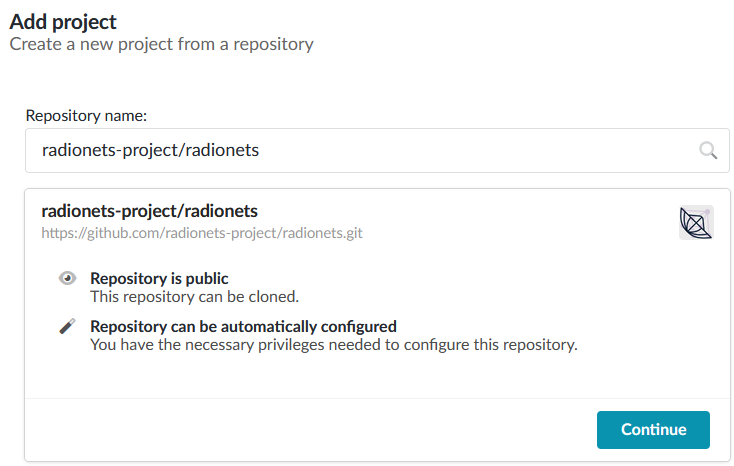
\includegraphics[width=\textwidth]{graphics/rtd2.png}
      }
      \only<4>{
        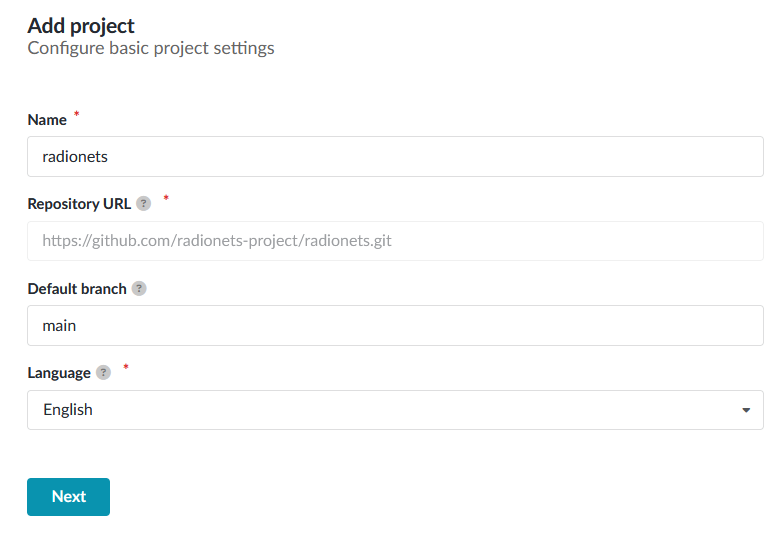
\includegraphics[width=\textwidth]{graphics/rtd3.png}
      }
      \only<5>{
        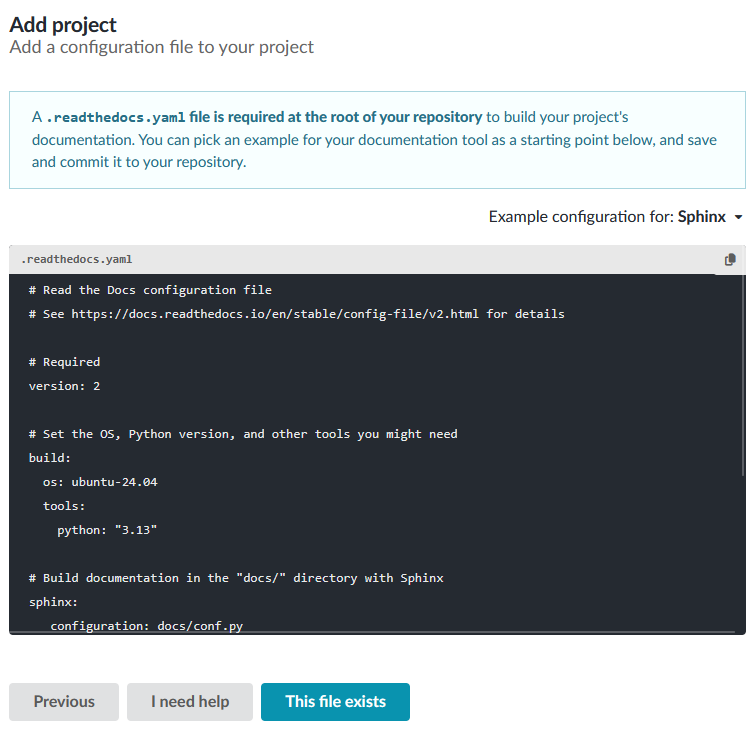
\includegraphics[width=\textwidth]{graphics/rtd4.png}
      }
      \only<6>{
        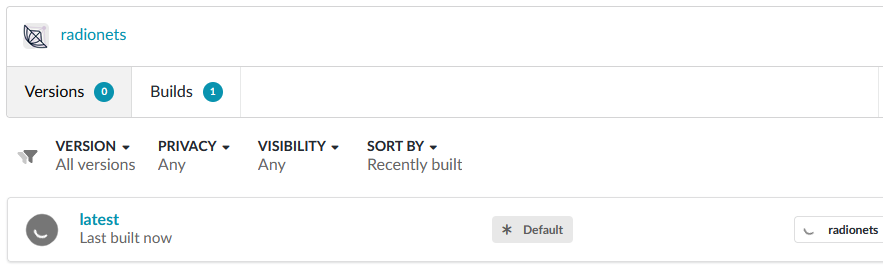
\includegraphics[width=\textwidth]{graphics/rtd5.png}
      }
    \end{column}
  \end{columns}
\end{frame}

\begin{frame}{Further Reading: Docs}
  \begin{columns}[t,onlytextwidth]
    \begin{column}{0.48\textwidth}
      \begin{itemize}
        \setlength{\itemsep}{1em}
        \item \iref{https://indico.desy.de/event/43817/sessions/19712/attachments/97983/135044/docs_ci_pyopp_2025.pdf}{My PYOPP Talk}
        \item \iref{https://www.sphinx-doc.org/en/master/}{Sphinx}
        \item \iref{https://github.com/sphinx-doc/sphinx-autobuild}{sphinx-autobuild}
        \item \iref{https://docs.python.org/3/reference/import.html}{Import System}
        \item \iref{https://peps.python.org/pep-0420/}{PEP 420 – Implicit Namespace Packages}
        \item \iref{https://www.sphinx-doc.org/en/master/usage/restructuredtext/basics.html}{reStructuredText (reST)}
        \item \iref{https://www.sphinx-doc.org/en/master/usage/restructuredtext/roles.html}{Roles}
        \item \iref{https://www.sphinx-doc.org/en/master/usage/restructuredtext/directives.html}{Directives}
      \end{itemize}
    \end{column}
    \begin{column}{0.48\textwidth}
      \begin{itemize}
        \setlength{\itemsep}{1em}
        \item \iref{https://www.sphinx-doc.org/en/master/usage/restructuredtext/field-lists.html}{Field Lists}
        \item \iref{https://towncrier.readthedocs.io/en/stable/index.html}{Towncrier} (Changelogs)
        \item \iref{https://sphinx-automodapi.readthedocs.io/en/latest/}{sphinx-automodapi}
        \item \iref{https://pydata-sphinx-theme.readthedocs.io/en/stable/}{PyData Sphinx Theme}
        \item \iref{https://numpydoc.readthedocs.io/en/latest/index.html}{numpydoc}
        \item \iref{https://sphinx-design.readthedocs.io/en/latest/}{sphinx-design}
        \item \iref{https://sphinx-gallery.github.io/stable/index.html}{sphinx-gallery}
      \end{itemize}
    \end{column}
  \end{columns}
\end{frame}
